% !TeX root = ../summary-syssec.tex

\section{Trusted Computing \& Attestation}
Acronyms:
\begin{description}
    \item[TCG] Trusted Computing Group
    \item[TPM] Trusted Platform Module
    \item[PCR] Platform Configuration Register
    \item[TCB] Trusted Computing Base
    \item[SRTM/DRTM] Static / Dynamic Root of Trust for Measurement
    \item[SLV] Secure Loader Block
    \item[TXT] Trusted Execution Technology
    \item[AIK] Attestation Identity Keys (for signing PCRs)
    \item[SRK] Storage Root Key
    \item[IEE] Isolated Execution Environment
    \item[DMA] Direct Memory Access
\end{description}

\subsection{Some Current Approaches}
\subsubsection{Program Code in ROM}
\begin{description}
	\item[Approach:] keep entire program in ROM
	\item[Advantage:] Simple, No injection possible
	\item[Disadvantage:] No updates possible, ROP attacks possible, no
	  isolation
	\item[Verdict:] Not practical
\end{description}

\subsubsection{Secure Boot}
\begin{description}
	\item[Approach:] Only load code with valid signature
	\item[Advantage:] Only approved software loaded
	\item[Disadvantage:] No isolation, difficult to prevent roll-back
	  attacks
	\item[Verdict:] Weak security guarantee
\end{description}

\subsubsection{Virtual-machine-based Isolation}
\begin{description}
	\item[Approach:] Isolate apps by executing in VM
	\item[Advantage:] smaller TCB, isolation between apps
	\item[Disadvantage:] VM still large \& part of TCB, complex
	\item[Verdict:] Step in right direction
\end{description}

\subsection{General Approach}
\begin{enumerate}
	\item Isolated Execution
	\item Remote Attestation
	\item Sealed Storage
\end{enumerate}

\subsection{TPM}
\subsubsection{Basics}
\begin{description}
    \item[Attestation] enables verifier to verify what SW is executing on untrusted device
\end{description}
Adversary model of TPM:
\begin{itemize}
    \item remote attacks
        \begin{itemize}
            \item compromise OS and apps running on the OS
            \item complete control over network communication
        \end{itemize}
    \item local hardware
        \begin{itemize}
            \item generally trusted (because HW attack detection is hard)
            \item attacker can reboot, install malicious SW, attack malicious USB devices
        \end{itemize}
\end{itemize}

Basic TPM functions
\begin{itemize}
    \item PCR registers for integrity measurement chain $PCR_{new} = \texttt{SHA-1}(PCR_{old}|| \texttt{SHA-1}(data))$
      \begin{itemize}
	\item Static PCRs are only reset at system boot.
	\item Dynamic PCRs initialized to -1 at system boot, reset to 0 upon entry into IEE.
      \end{itemize}

    \item on-chip storage for SRK
    \item manufacturer certificate
    \item remote attestation with PCRs and AIK
    \item sealed storage with PCRs and SRK (only accessible under certain integrity measurement)
    \item random number generator
\end{itemize}
TPM is \textbf{passive} component and \textbf{not} tamper proof.

HW attacks possible because TPM is on LPC bus.

\subsubsection{Attested Boot a.k.a. Static Root of Trust}
Measure all executed SW to verify platform configuration. To verify compare measurements to known hashes of trusted SW.

Shortcomings:

\begin{itemize}
    \item TOCTTOU: measurement at load-time and not at runtime (inefficient against dynamic attacks)
    \item coarse-grained: TCP is entire system
    \item no guarantee of execution
    \item every system is different $\Rightarrow$ Database of correct hashes is
      large
\end{itemize}

\subsubsection{Dynamic Root of Trust a.k.a. Late Launch}
Idea: special CPU instruction to create IEE $\xrightarrow{}$ high assurance of code execution and remote attestation

Required computing primitives:
\begin{itemize}
    \item create IEE with \texttt{SKINIT/SENTER}
        \begin{enumerate}
            \item CPU softreset
            \item reset dynamic PCRs
            \item enable DMA protection
            \item send SLB to TPM
            \item execute SLB
        \end{enumerate}
    \item remote attestation
      \begin{center}
	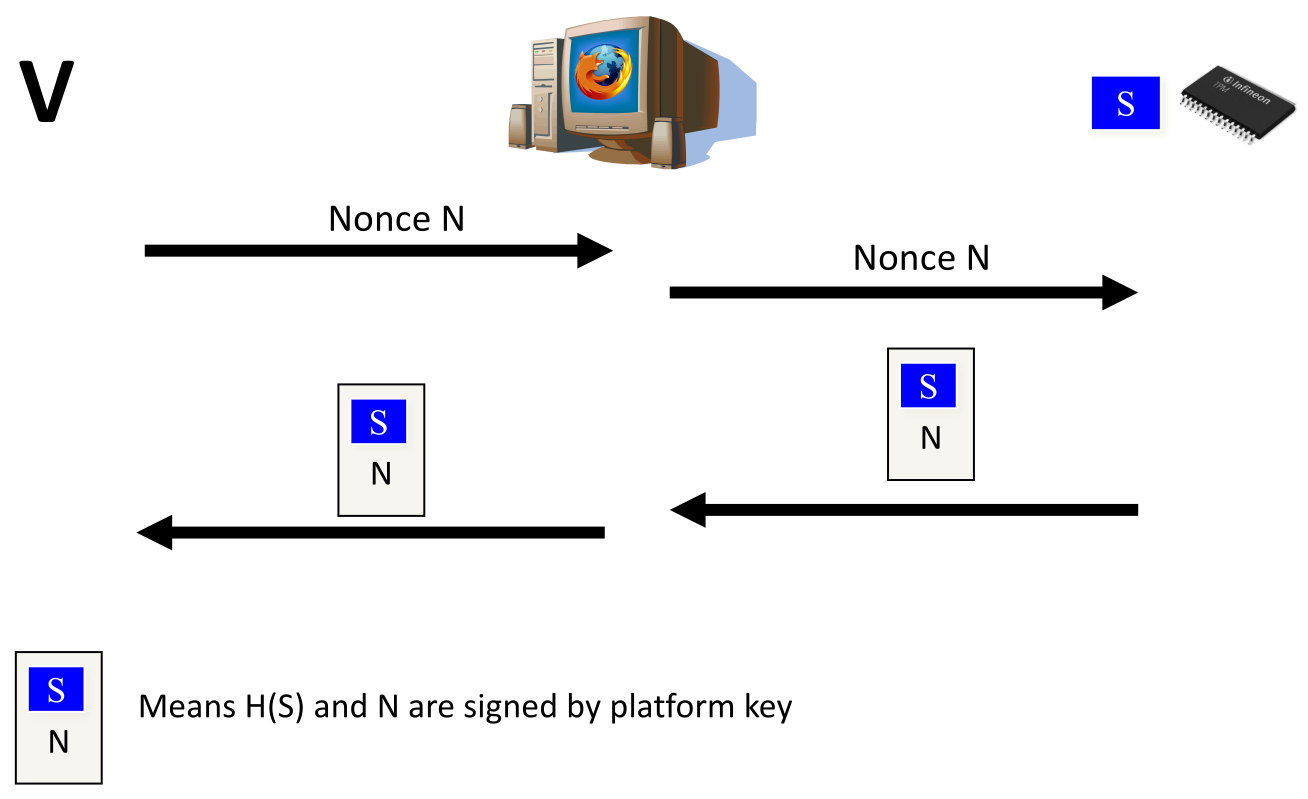
\includegraphics[width=0.8\columnwidth]{tcg-attestation.png}
      \end{center}
        \begin{enumerate}
            \item verifier sends nonce to TPM
            \item TPM returns measurements, nonce signed with platform key
        \end{enumerate}
	\textbf{Attestation says, that \textit{a} TPM signed it, but not
	\textit{which}} $\Rightarrow$ Possible attack!
    \item establish secure channel
      \begin{center}
	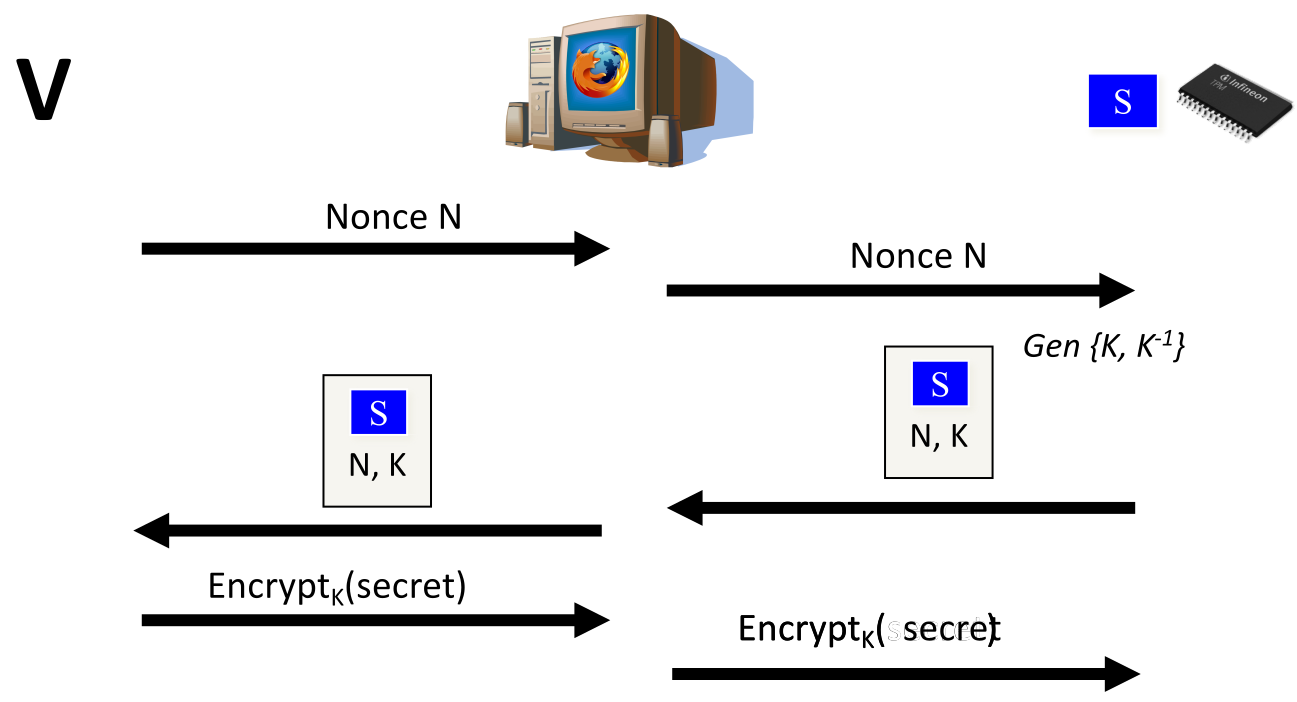
\includegraphics[width=0.8\columnwidth]{tcg-secure-channel.png}
      \end{center}
        \begin{enumerate}
            \item verifier sends nonce to TPM
            \item TPM generates $\{K, K^{-1}\}$, send back $\{\texttt{measurement, nonce}, K\}$ signed with platform key
        \end{enumerate}
    \item verify output
      \begin{center}
	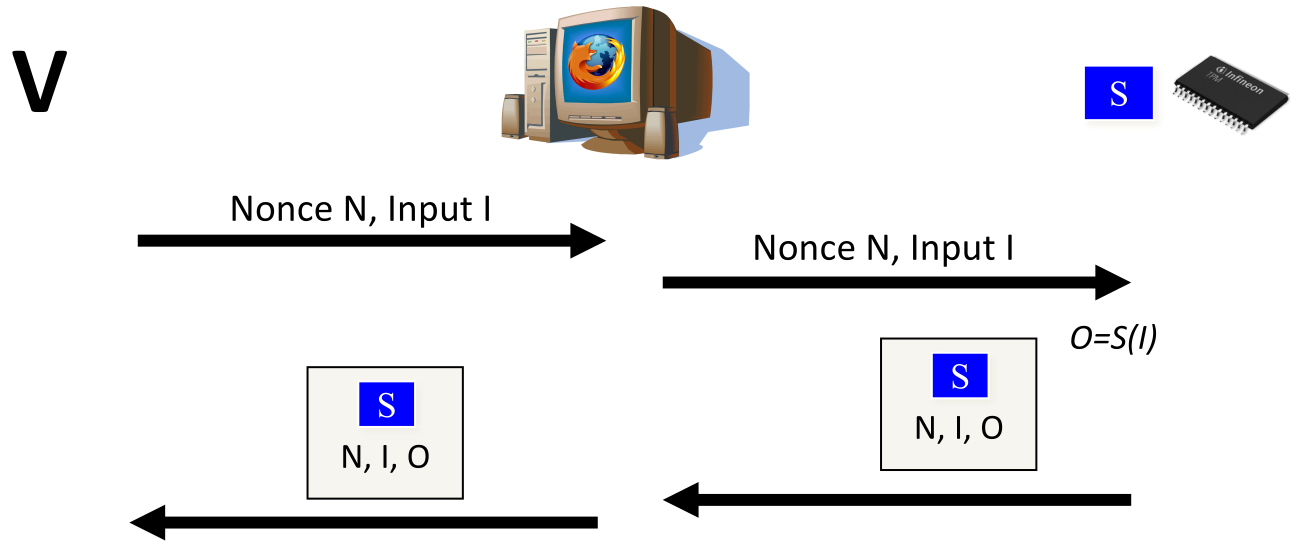
\includegraphics[width=0.8\columnwidth]{tcg-io.png}
      \end{center}
        \begin{enumerate}
            \item verifier sends nonce to TPM
            \item TPM sends back measurement, nonce, input and output signed with platform key
        \end{enumerate}
\end{itemize}

\textbf{No need to trust OS anymore, therefor minimal TCB.}

\subsection{SGX vs TPM}
SGX advantages:
\begin{itemize}
    \item Memory encryption
    \item robust against LPC-bus tampering
    \item can execute unprivileged code (ring 3)
    \item multi-threaded execution
    \item parallel execution of enclave and untrusted code
    \item enclaves can be interrupted
\end{itemize}

SGX disadvantages:
\begin{itemize}
    \item no sealed storage
    \item remote attestation requires online third party (Intel)
    \item memory access pattern reveals information about computation
\end{itemize}
